\chapter{Integration over Hybrid Domains}
\label{chp:Integration}


%%%%%%%%%%%%%%%%%%%%%%%%%%%%%%%%%%%%%%%%%
%
% INTRODUCTION
%
%%%%%%%%%%%%%%%%%%%%%%%%%%%%%%%%%%%%%%%%%

In many ways, integration provides the inspiration for hybrid set domains.
As such, many of the techniques we have been using will be very familiar when placed back within their original context.
That being said, notationally, sets and orientation are treated as often treated as distinct objects rather than a single entity.


As a hopefully illustrative example of this, consider a typical definition of the \textbf{definite integral} from an introductory
course in calculus.
Given a function $f$ with real variable $x$ and an interval $[a,b)$ of the (extended) real line
\footnote{ The extended real line denoted $\extendedreal$ is the set of real numbers as well as the points at 
$+\infty$ and $-\infty$} the definite integral
\begin{equation*}
	\int_a^b f(x) \diff x
\end{equation*}
is defined as the signed area bounded by $f$ between $x=a$ and $x=b$.
Generally after a short exposition about Riemann sums, it would then be revealed that if $F$ is an anti-derivative of the
 function $f$ then:
\begin{equation*}
	\int_a^b f(x) \diff x \;=\; F(b)-F(a) \;=\; - (F(a)-F(b)) \;=\; - \int_b^a f(x) \diff x
\end{equation*}


However this means that previously defining the definite integral using (unoriented) intervals was a bit of a misnomer.
As we saw in the previous chapter, when $a \geq b$, the interval $[a,b) = \{ x \;|\; a \leq x < b \}$ is the empty set.
So the interval itself cannot really be thought of as a part of the definite integral.
If it were the interval itself that we were concerned with then for $a \leq b$, the interval $[b,a)$ is empty.
As are the intervals $[a,a)$, $[\pi, e)$, and$[\infty, -\infty)$.
As these are all different representations of the same interval, and we are considered with the relationship between $f$ and
the interval, then one might argue that, in fact
\begin{equation*}
	\int_b^a f(x) \diff x \;=\; \int_a^a f(x) \diff x \;=\; \int_\pi^e f(x)\diff x \;=\; \int_\infty^{-\infty} f(x) \diff x
\end{equation*}
Obviously this is not the intent but there is a distinct mismatch between the conceptual usefulness of considering
integrals as over an interval.
But when actually using said interval, it is treated as an ordered pair of endpoints disregarding the set itself.


This issue is exasperated working with the more general notation
\begin{equation*}
	\int_X f(x) \diff x
\end{equation*}
which denotes integrating $f$ over a set $X$.
Now there is nothing stopping $X$ from an interval and one would very much like to say that we can convert between the
two notations with a definition like:
\begin{equation*}
	\int_a^b f(x) \diff x \;=\; \int_{[a,b)} f(x) \diff x
\end{equation*}
but there is no analogous translation to $\int_a^b = - \int_b^a$ and so if we made this assertion we would be left with
\begin{equation*}
	\int_{[a,b)} f(x) \diff x 
		= \int_a^b f(x) \diff x 
		= -\int_b^a f(x) \diff x 
		= - \int_{[b,a)} f(x)\diff x 
		= -\int_\emptyset f(x)\diff x 	
		= 0
\end{equation*}
This is clearly not a desired outcome; instead what is actually intended is an oriented interval.
The integral should instead be over the hybrid set $[\![a,b)\!)$.



Another advantage to using oriented sets is a more natural language for manipulating domains of integration than sets.
We cannot add sets (in the traditional, non-$\sigma$-algebra sense) 
but with the point-wise sum $\oplus$, we \emph{can} add hybrid sets.
This allows us to say that the integral operator is \emph{bi-linear}.
By this we mean, that integration is a function of two operands, the integrand and the domain.
Integration is linear over integrands regardless,
\begin{equation}
	\int_{X} f(x) + g(x) \diff x = \int_X f(x) \diff x + \int_X g(x) \diff x
\end{equation}
but with summation defined on the domain as well
\begin{equation}
	\int_{X\oplus Y} f(x) \diff x = \int_{X} f(x) \diff x + \int_Y f(x) \diff x
\end{equation}


In one dimension, many of these changes may seem trivial advances but in higher dimensions, 
the oriented and measure-theoretic approaches diverge \cite{tao2007differential}.
A Riemann integration foundation is not overly concerned with negatively oriented intervals and the definitions continue
to function unperturbed by the fact that the ``right-hand'' bound is actually less than the ``left-hand'' bound.
As such extending to higher dimension Riemann integrals, orientation is easily bundled in as well.
But measure-based approaches to integration need to fake orientation in one dimension.
First one must convert $\int_a^b$ into either $-\int_{[a,b)}$ or $\int_{[a,b)}$ and then integrate one or the other.
Once one commits to an orientation, there is no coming back.
In higher dimensions, this becomes more of a problem.

This is usually forgivable given the extra power the Lebesgue integral affords over the Riemann.
Using hybrid sets as domains of integration allow us to use the best features of both.
In this chapter we will investigate integration using hybrid set domains.




%%%%%%%%%%%%%%%%%%%%%%%%%%%%%%%%%%%%%%%%%
%
% HYBRID INTEGRATION
%
%%%%%%%%%%%%%%%%%%%%%%%%%%%%%%%%%%%%%%%%%



%%%%%%%%%%%%%%%%%%%%%%%%%%%%%%%%%%%%%%%%%
% RIEMANN
%%%%%%%%%%%%%%%%%%%%%%%%%%%%%%%%%%%%%%%%%
\section{The Riemann Integral on $k$-rectangles}

\begin{definition}
	Let $[\![\boldsymbol{a}, \boldsymbol{b}]\!]$ be a $k$-rectangle in $\mathbb{R}^n$ 
	where $\boldsymbol{a}=(a_1,\ldots, a_n)$ and $\boldsymbol{b}=(b_1,\ldots, b_n)$. 
	We denote the \textbf{volume of $\boldsymbol{[\![a,b]\!]}$} with $\text{vol}$ and define it as:
	\begin{equation}
		\vol(\; [\![\boldsymbol{a}, \boldsymbol{b} ]\!] \;) 
			= (b_1 - a_1) \cdot (b_2 - a_2) \cdot \ldots \cdot (b_n - a_n)
	\end{equation}
\end{definition}

We say volume, but this depends on the dimension.
In 2-dimensions, this would better be described as area and in 1-dimension as a length.
For any $k<n$, a $k$-rectangle will have volume zero.
This is fitting, as we wished for example to measure the area of rectangle in 2 dimensions, but the same 2-rectangle in
$\mathbb{R}^3$ is flat and can hold no volume.
In at least one dimension, the cube will be degenerate (i.e. $a_i = b_i$) and so will contribute zero to the product.
Additionally, one can also observe that $\text{vol}( \ominus [\![\boldsymbol{a}, \boldsymbol{b} ]\!]) 
= - \text{vol}( [\![ \boldsymbol{a}, \boldsymbol{b} ]\!] )$.


The next task is to partiton the $k$-rectangle $[\![\boldsymbol{a}, \boldsymbol{b}]\!]$ into a grid of smaller
$k$-rectangles.
To do this, for each dimension $[\![a_i, b_i]\!]$, we choose a generalized partition $P_i$ such that $P_i$ is composed of
oriented intervals.
To build our mesh, we construct smaller $k$-rectangles $I_{i_1, \ldots, i_n}$ using the Cartesian product of pieces:
\begin{equation}
	I_{p_1, \ldots, p_n} = p_1 \times \ldots \times p_n
\end{equation}
where each $p_i$ is taken from $P_i$.
We are now ready to construct Riemann sums.

\begin{definition}
	Given $P=\{ P_j \}_{j=1}^n$ where $P_j$ is an interval generalized partition of $[\![a_j, b_j]\!]$,
	and $f:[\![\boldsymbol{a}, \boldsymbol{b}]\!] \to \mathcal{R}$ then we define a Riemann sum $f_P$ to be:
	\begin{equation}
		f_P = \sum_{p_1 \in P_1} \ldots \sum_{p_n \in P_n} f(x^*_{p_1, \ldots, p_n}) \vol(I_{p_1, \ldots, p_n})
	\end{equation}
	where $x^*_{p_1, \ldots, p_n}$ is any point chosen from $I_{p_1, \ldots, p_n}$.
\end{definition}

Note that we specify \emph{a} Riemann sum, not \emph{the} Riemann sum.
There are several ways to choose $x^*_{i_1,\ldots,i_n} \in I_{i_1, \ldots, i_n}$ and different samplings can lead to different Riemann sums for the same partition and same function.
In $\mathbb{R}^1$, several common ways to sample include the left and right Riemann sums (which sample at the left and right boundaries), the trapezoidal Riemann sum (which averages the left and right) the upper Riemann sum (which samples at $\max(f(x_{i_1, \ldots, i_n}))$) and the lower Riemann sum (which samples at $\min(f(x_{i_1,\ldots,i_n}))$).


\begin{figure}[ht]
\caption[Riemann Integral]{Upper and lower Riemann sums shown for the same sequence shown with light and dark rectangles respectively. A function over an oriented interval is Riemann integrable if the two sums converge.}
\centering
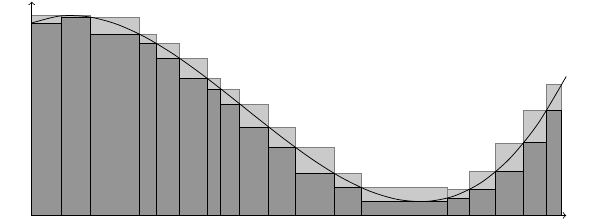
\includegraphics[scale=0.6]{diagrams/riemann}
\end{figure}


\begin{definition}
The Riemann integral of a function $f:\mathbb{R}^n \to \mathbb{R}$ over a $k$-rectangle 
$[\![\boldsymbol{a}, \boldsymbol{b}]\!]$ as $\max( | \vol( I_{p_1,\ldots, p_n}) | : p_i \in P_i )$ goes to zero.
	\begin{equation}
		\int_{[\![a,b]\!]} f(x) \diff x = f_P
	\end{equation} 
	We say that a function is \textbf{Riemann integrable} if the upper and lower Riemann sums converge.
\end{definition}






%%%%%%%%%%%%%%%%%%%%%%%%%%%%%%%%%%%%%%%%%
% LEBESGUE INTEGRAL
%%%%%%%%%%%%%%%%%%%%%%%%%%%%%%%%%%%%%%%%%
\section{The Lebesgue Integral on hybrid domains}

Another common approach to integration is the Lebesgue integral which approaches integration from a measure theoretic
perspective.
We begin our construction with a $\sigma$-algebra (read sigma-algebra) over a set $X$.
By this we mean a collection of subsets of $X$ which are closed under countable complement, union and intersection.
The important part here is that we have a closed universe of sets on which we can perform 
\emph{nearly} arbitrary set operations but remain within said universe.
Next we can attach to a $\sigma$-algebra a measure to form a \textbf{measure space} $(X, \Sigma, \mu)$ 
where $X$ is a set $\Sigma$ is a $\sigma$-algebra  over subsets of $X$ and $\mu$ is a measure defined on the sets in
 $\Sigma$.
This measure $\mu$ is a function $\mu: \Sigma \to \extendedreal$ with the following properties:
\begin{description}
	\item[Non-negative:] For all $E \in \Sigma$, $\mu(E) \geq 0$
	\item[Empty set has measure 0:] $\mu(\emptyset) = 0$
	\item[Countably Additive:] For $\{E_i\}_i$, a countable set of disjoint sets in $\Sigma$,
		$\mu \left( \bigcup_i E_i \right) = \sum_i \mu(E_i)$
\end{description}
Within the context of integration, the Borel and Lebesgue measure spaces are notable constructions.
Both of which give a suitably large universe of sets for which to integrate over.
Certainly much more than the set of Riemann integrable domains.
Finally, given a measure space $(X, \Sigma, \mu)$, we say that $f : X \to \mathbb{R}$ is a \textbf{measurable function}
if  $\{ x \; | \; f(x) > t\}$ is a measurable set for all $t$.



If $\ind[S]$ is indicator function $\ind[S] : X \to \{ 0, 1 \}$ given by 
$\ind[S] (x) = 1$ if $x \in S$ and $\ind[S] (x) = 0$ otherwise.
Clearly if $S$ is a measurable set, then $\ind[S]$ is a measurable function.
We will use this as a base case.
Given a measure space $(X, \Sigma, \mu)$ and $S \in \Sigma$, we define the integral:
\begin{equation}
	\int \! \ind[S] \diff \mu = \mu ( S )
\end{equation}


From this, we consider functions which are the sum of indicator functions.
We say that $s$ is a \textbf{simple function} if there are finite sets of measurable sets and $\{ A_k \}_{k=0}^n$
and matching real coefficients $\{ a_k \}_{k=0}^n$ such that:
\begin{equation}
	s = \sum_{k=0}^n a_k \ind[A_k]
\end{equation}
The integral of a simple function is then easily defined linearly in terms of integrals of indicator functions:
\begin{equation}
	\int \! s \diff \mu 
		= \int \left(\sum_{k=0}^n a_k \ind[A_k] \right) \diff \mu 
		= \sum_{k=0}^n a_k  \int \! \ind[A_k] \diff \mu
		= \sum_{k=0}^n a_k \cdot \mu(A_k)
\end{equation}

But we don't always wish to integrate over the entire measure space but rather some measurable subset of $X$.
This would be done with the notation $\int_B$ instead of $\int$ and replacing $\mu(A_k)$ with $\mu(A_k \cap B)$.
If $A_k$ and $B$ are both measurable sets in $\Sigma$ then their intersection is also a measurable set in $\Sigma$.
But as already mentioned, integrating over sets is a misnomer; we should be integrating over oriented sets.
To do this, we extend $\mu$ linearly for hybrid sets on $\Sigma$.
Strictly speaking, doing so means that $\mu$ is no longer a measure as it takes on negative values.
For a hybrid set $H \in \hsetover[\Sigma]$,
\begin{equation}
	\int_H s \diff \mu = \int H \cdot s \diff \mu = \sum_k a_k \cdot \mu(A_k \otimes H)
\end{equation}


We then use simple functions to approximate general measurable functions.
For a non-negative function $f$, we say this is the largest simple function that is everywhere less than $f$:
\begin{equation}
	\int_H \! f \diff\mu = 
		\text{sup} \left\{ 
			\int_H s \diff \mu \;\middle|\; s \text{ simple, and } 0 \leq \varphi \leq f 
		\right\}
\end{equation}
But even if $f$ takes negative values, we can split it into positive and negative parts by:
\begin{align}
f^+(x) &:= \mathrm{max}( 0, f(x)) \\
f^-(x) &:= \mathrm{max}(0, -f(x)) 
\end{align}
Both $f^+$ and $f^-$ are clearly non-negative but also, observe that $f=f^+ - f^-$.
Linearly, this allows us to define for any measurable $f$:
\begin{equation}
\int_H f \diff \mu = \int_H f^+ \diff \mu - \int_H f^- \diff \mu
\end{equation}


The last issue that remains to be settled is whether such a limit even exists.
For this we can use the sequence of simple functions $\psi_n$ defined by:
\begin{equation}
	\psi_n = \sum_{k=0}^{n2^n -1} 
		\left[ \left(\frac{k}{2^n}\right)^{\left[ \frac{k}{2^n}, \frac{k+1}{2^n} \right)} \right] 
		+ n^{[n,\infty]}
\end{equation}
Notationally, this definition is rather heavy but is easily understood geometrically as seen below in
Figure~\ref{fig:simplefunc}.
In turn this allows us to define for any non-negative $f$ the sequence of functions  $\varphi_n = \psi_n \circ f$.
We know that $\varphi_n$ is simple since $\psi_n$ is simple.
And since $\psi_n(x) \leq x$ for all $x$ then we also have $0 \leq \varphi_n \leq f$.
But, most importantly we have $0 \leq f(x) - \varphi_n(x) \leq 2^{-n}$ and 
so $\varphi_n$, uniformly approaches $f$ as $n$ approaches infinity. 
\begin{figure}[ht]
	\caption[Approximations using simple functions]{
	The simple functions $\psi_n$ for $n$ from $1$ to $4$.
	As $n$ goes to infinity, $\psi_n$ comes arbitrarily close to $x$ over the range 0 to $n$.
	}
	\label{fig:simplefunc}
	\centering
	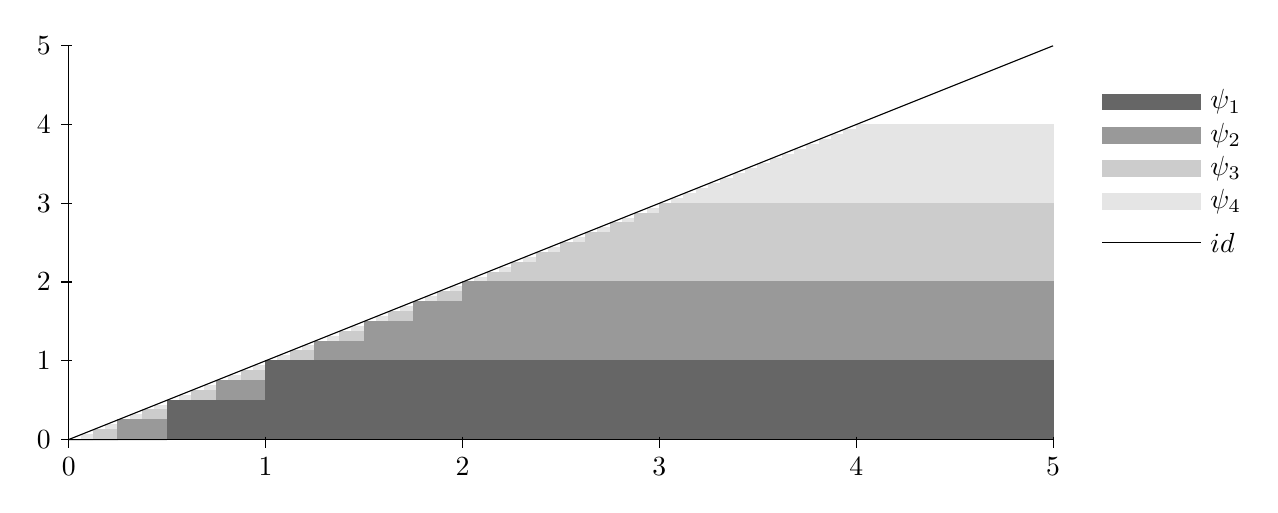
\begin{tikzpicture}[y=1cm, x=2.5cm]
		%psi 4
		\foreach \x in {0,0.0625,...,3.99}
			\draw[fill, color=black!10] (\x,0) rectangle ++ (0.0625, \x);
		\draw[fill, color=black!10] (4,0) rectangle (5,4);
		%psi 3
		\foreach \x in {0,0.125,...,2.9}
			\draw[fill, color=black!20] (\x,0) rectangle ++ (0.125, \x);
		\draw[fill, color=black!20] (3,0) rectangle (5,3);
		%psi 2
		\foreach \x in {0,0.25,...,1.9}
			\draw[fill, color=black!40] (\x,0) rectangle ++ (0.25, \x);
		\draw[fill, color=black!40] (2,0) rectangle (5,2);
		%psi 1
		\foreach \x in {0,0.5,...,0.9}
			\draw[fill, color=black!60] (\x,0) rectangle ++ (0.5, \x);
		\draw[fill, color=black!60] (1,0) rectangle (5,1);
	 	%axis
		\draw(0,0) -- coordinate (x axis mid) (5,0);
	    	\draw (0,0) -- coordinate (y axis mid) (0,5);
	    	%ticks
	    	\foreach \x in {0,1,...,5}
	     		\draw (\x,1pt) -- (\x,-3pt)
				node[anchor=north] {\x};
	    	\foreach \y in {0,1,...,5}
	     		\draw (1pt,\y) -- (-3pt,\y) 
	     			node[anchor=east] {\y}; 
	     	% y= x		
		\draw (0,0) -- (5,5);
		%legend
		\begin{scope}[shift={(5.25,2.5)}] 
			\draw[yshift=4\baselineskip, fill, color=black!60] (0,0) rectangle (0.5,0.2) --++ (0,-0.1)
				node[right, color=black]{$\psi_1$};
			\draw[yshift=3\baselineskip, fill, color=black!40] (0,0) rectangle (0.5,0.2) --++ (0,-0.1) 
				node[right, color=black]{$\psi_2$};	
			\draw[yshift=2\baselineskip, fill, color=black!20] (0,0) rectangle (0.5,0.2) --++ (0,-0.1) 
				node[right, color=black]{$\psi_3$};
			\draw[yshift=\baselineskip, fill, color=black!10] (0,0) rectangle (0.5,0.2) --++ (0,-0.1) 
				node[right, color=black]{$\psi_4$};
			\draw (0,0) -- (0.5,0) node[right] {$id$};
		\end{scope}
	\end{tikzpicture}
\end{figure}








%%%%%%%%%%%%%%%%%%%%%%%%%%%%%%%%%%%%%%%%%
% ''HAVING YOUR CAKE AND EATING IT TOO'' EXAMPLE
%%%%%%%%%%%%%%%%%%%%%%%%%%%%%%%%%%%%%%%%%
\subsection{Example: \emph{Integrating the Irrationals}}

A Lebesgue measurable hybrid set can now have an orientation like Riemann integral intervals 
and the power of Lebesgue integration.
Consider the indicator function for the set of rational numbers, $1_\mathbb{Q}$ which evaluates to 
1 for rational numbers and 0 for irrational numbers.
Over the interval $[0,1]$ on the real line, this is not Riemann-integrable.
Suppose we have some generalized partition of $[0,1]$ made up of intervals.
Then for any of these sub-intervals, there will be at least one rational and one irrational number.
Hence the upper Riemann sum will be 1 and the lower Riemann sum will be 0.
No matter how small we make our intervals, there will always be a rational and irrational number in each.
The two sums will never converge and so there is no well-defined Riemann integral.


On the other hand, it is Lebesgue integrable:
\begin{equation}
	\int_{[0,1]} 1_\mathbb{Q} \diff\mu = \mu(\mathbb{Q} \cap [0,1])
\end{equation}
But since $\mathbb{Q}$ is countable, it has measure 0 and so $1_\mathbb{Q}$ \emph{is} Lebesgue integrable on $[0,1]$.
Similarly, we could also find that:
\begin{equation}
	\int_0^1 1_{\mathbb{R}\setminus \mathbb{Q}} \diff \mu
		= \int_{[0,1]} 1_{\mathbb{R}\setminus \mathbb{Q}} \diff \mu
		= \mu \big( (\mathbb{R}\setminus\mathbb{Q}) \cap [0,1] \big)
		= \mu \big( (\mathbb{R}\setminus\mathbb{Q}) \cap [0,1] \big)
		= 1
\end{equation}

One would expect the same process to hold for when integrating from 0 to 1 but restricted to sets, this is not possible.
The statement $[1,0] = -[0,1]$ is nonsense.
But if we instead take integrating from $a$ to $b$ to mean the Lebesgue integral over the oriented $[\![a,b]\!]$.
Additionally instead of the Lebesgue measure $\mu$ which is defined for 
measure $\nu$:

\begin{equation}
	\int_1^0 1_{\mathbb{R}\setminus \mathbb{Q}} \diff \nu
		\;=\; \int_{[\![0,1]\!]} 1_{\mathbb{R}\setminus \mathbb{Q}} \diff \nu
		\;=\; \nu \big( (\mathbb{R}\setminus\mathbb{Q} ) \otimes [\![1,0]\!] \big)
		\;=\; -1
\end{equation}

%%%%%%%%%%%%%%%%%%%%%%%%%%%%%%%%%%%%%%%%%
% DIFFERENTIAL FORMS
%%%%%%%%%%%%%%%%%%%%%%%%%%%%%%%%%%%%%%%%%

\section{Differential Forms}

Rather than thinking of integrals as functions over $n$-rectangles, an often more useful language is to use 
\emph{differential forms}.
We define a \textbf{(differential) 0-form} $\beta$ on $\mathbb{R}^n$ as any function 
$\beta : \mathbb{R}^n \to \mathbb{R}$.
And there is very little else to say as they are just functions on $\mathbb{R}^n$.



A \textbf{(differental) 1-form} $\omega$ on $\mathbb{R}^n$ is an expression of the form:
\begin{equation}
	\omega = f_1(\text{x}) \diff x_1 + f_2(\text{x}) \diff x_2 + \ldots + f_n(\text{x}) \diff x_n
\end{equation}
Now this look very much like something we're used to integrating.
Specifically it is something that be used as an integrand over a 1 dimensional domain.
For example, Green's theorem is introduced using differential forms without even mentioning them as such.
\begin{equation}
	\tag{Green's Theorem}
	\textcolor{black!40}{
		\int_D \left( \frac{\partial f_2}{\partial x} - \frac{\partial f_1}{\partial y}  \right) \diff x \diff y 
		=\int_{C}
	} f_1(x,y) \diff x + f_2(x,y) \diff y
\end{equation}
Here $C$ is a closed curve that encloses $D$ a region in the $(x,y)$ plane; hence the right-hand side is an integral of
a 1-form over a 1-dimensional curve.
Having multiple $\diff x_i$ appearing in a single integrand may initially seem unusual when first presented, 
but is quite intuitively handled.
Integration is linear so just as we can separate $\int f(x) + g(x) \diff x$ into $\int f(x) \diff x + \int g(x) \diff x$, 
we can similarly breakup an integral of a 1-form into the sum of integrals over \emph{basic} 1-forms 
(1-forms involving a single term).
\begin{equation}
	\int f_1(\text{x}) \diff x_1 
		+ f_2(\text{x}) \diff x_2 
		+ \ldots 
		+ f_n(\text{x}) \diff x_n
	=	\sum_{i=1}^n \left( \int f_i \diff x_i \right)
\end{equation}


Adding two 1-forms then is quite straight-forward; simply collect terms with matching $dx_i$.
So if we can add differential forms but what about multiplication?
For a 0-form $\beta$ and 1-form $\omega$ as defined above, the answer the answer is a simple yes:
\begin{equation}
	(\beta \cdot \omega)(\text{x}) 
		= \beta(\text{x})f_1(\text{x}) \diff x_1 
		+ \ldots  
		+ \beta(\text{x})f_n(\text{x}) \diff x_n
\end{equation}
The result is a 1-form where each basic 1-form term is the product of $f_i$ and $\beta$ in $\mathbb{R}$.
To ``multiply'' two 1-forms together however we must turn instead to the wedge product $\wedge$.

First of all, the wedge product is primarily defined by being \emph{anti-commutative} or \emph{skew-symmetric}.
That is, $\diff x \wedge \diff y = -\diff y \wedge \diff x$ and several results will immediately follow.
When applied to two identical $dx$, we have $\diff x \wedge \diff x = - \diff x \wedge \diff x$ 
and so $\diff x \wedge \diff x = 0$.
Additionally, for any permutation $\sigma$ of $[p]$
\begin{equation}
	\diff x_1 \wedge ... \wedge \diff x_p 
	= \text{sgn}(\sigma) \diff x_{\sigma(1)} \wedge ... \wedge \diff x_{\sigma(p)}
\end{equation}
The wedge product of two 1-forms moves us out of the realm of 1-forms which have basis $\diff x_i$ and into the 
realm of 2-forms with basis $\diff x_i \wedge \diff x_j$.


\begin{definition}
	Given a $k$-rectangle $\Omega \in \mathbb{R}^n$ with coordinates $\text{x} = (x_1, x_2, \ldots, x_n)$
	A \textbf{differential $p$-form} $\beta$ over $\Omega$ has the form:
	\begin{equation}
		\beta = \sum_{j_1 \in [n]} \ldots \sum_{j_p \in [n]} b_{(j_1, \ldots, j_p)}(\text{x})
				\diff x_{j_1} \wedge \ldots \wedge \diff x_{j_p}
	\end{equation}
	Typically, we will take $j$ to be the vector $(j_1, \ldots, j_p)$ 
	and express $\beta$ instead as a single sum multi-indexed
	by $j$, $\sum_j b_j(x) \; dx_{j_1} \wedge \ldots \wedge dx_{j_p}$.
	We denote the space of all $p$-forms on $\Omega$ by $\Lambda^p(\Omega)$.
\end{definition}


\begin{definition}
	Let $\alpha = \sum_i a_i(x) \diff x_{i_1} \wedge \ldots \wedge \diff x_{i_p} \in \Lambda^p(\Omega)$ 
	and $\beta = \sum_j b_j(x) \diff x_{j_1} \wedge \ldots \wedge \diff x_{j_q} \in \Lambda^q(\Omega)$. 
	We extend the wedge product to 
	$\wedge : \Lambda^p(\Omega) \times \Lambda^q(\Omega) \to \Lambda^{p+q}(\Omega)$ by:
	\begin{equation}
		\alpha \wedge \beta  = \sum_{i,j} a_i(x) b_j(x)
			\diff x_{i_1} \wedge \ldots \wedge \diff x_{i_p} \wedge 
			\diff x_{j_1} \wedge \ldots \wedge \diff x_{j_q}
	\end{equation}
\end{definition}

Although we take all possible $\binom{n}{q} \cdot \binom{n}{p}$ pairs of 
$a_i (x) \diff x_{i_1} \wedge \ldots \wedge \diff x_{i_p}$ and $b_i (x) \diff x_{i_1} \wedge \ldots \wedge \diff x_{i_p}$,
most of the possible terms will end up being zero.
If \emph{any} of the terms in $\diff x_{i}$ appears in $\diff x_{j}$, then the wedge product will be zero 
and no term will be contributed.
As such, if $q+p > n$, there will be a duplicate in every term and so the entire sum will be zero.
When all is said and done, at most we will have $\binom{n}{p+q}$ terms.
Rather than the skew-symmetry we had when commuting $\diff x \wedge \diff y$, 
in higher dimensions the sign depends on $p \cdot q$ of the $p$-form and $q$-form we are commuting.
Specifically, 
\begin{equation}
	\alpha \wedge \beta = (-1)^{pq} \beta \wedge \alpha
\end{equation}
This can be easily seen by commuting each of $\diff x_{j_1}, \ldots \diff x_{j_q}$ terms each past 
$\diff x_{i_1}\wedge \ldots \wedge \diff x_{i_p}$. 
So we are commuting $q$ terms each past $p$ terms, reversing the sign each time for a net $(-1)^{pq}$.


The wedge product is only one part of our algebra of differential forms.
We have several other nice identities for its behaviour with addition and multiplication.
For the following, we consider $f$ to be a function on $\mathbb{R}^n$.
Additionally we consider the differential forms $\omega_1$ and $\omega_2$ to be $k$-forms, 
$\alpha$ to be a $p$-form and $\beta$ to be an $q$-form.
Then we have the following:
\begin{align}
	(\omega_1 + \omega_2) \wedge \alpha  & \;=\; \omega_1 \wedge \alpha + \omega_2 \wedge \alpha \\
	(\omega_1 \wedge \alpha) \wedge \beta & \;=\; \omega_1 \wedge ( \alpha \wedge \beta ) \\
	(f \cdot \omega_1) \wedge \alpha & \;=\;  f \cdot (\omega_1 \wedge \alpha) \;=\; \omega_1 \wedge (f \cdot \alpha)
\end{align}
These should all be quite obvious from definitions. 
We should also note the identities which are \emph{not} present.
We have defined the sum of $\omega_1$ and $\omega_2$: two differential forms which are the same dimension but not
the sum of $\alpha$ and $\beta$: differential forms with different dimension.
It is clear how one would add two differential forms of the same dimension as both were defined as sums to begin with.
We also do not define the multiplication of $\cdot$ two differential forms but we multiplying a form by a function is simply:
\begin{equation}
	(f \cdot \alpha) (x) = \sum_i f(x)\cdot a_i(x) \diff x_{i_1} \wedge \ldots \wedge \diff x_{i_p}
\end{equation}


Integrating over a $k$-form is quite simple.
First we shall consider integrating a $k$-form over a $k$-rectangle in $\mathbb{R}^k$.
Such a $k$-form is also known as a \emph{top-dimensional form}.
As we saw previously, any form of higher degree must be zero.
If $\omega$ is such a top form then we can always write
\begin{equation}
	\omega = f \; \diff x_1 \wedge \ldots \wedge \diff x_k
\end{equation}
for some function $f$.
Other presentations of $\omega$ exist, but we can always achieve such a presentation by commuting over $\wedge$ 
to the canonical ordering $x_1, \ldots, x_n$.
Once we have the $k$-form in this presentation, we just remove the wedges and evaluate the integral using the
integrand $f \diff x_1 \diff x_2 \ldots \diff x_k$.

\begin{definition}
	Let $\alpha$ be a $k$-form on $\Omega \subset \mathbb{R}^n$ of the form 
	$\alpha = A(x) \diff x_1 \wedge ... \wedge \diff x_n$.
	If $A \in \mathcal{L}^1 (\Omega , \diff x)$ then we define:
	\begin{equation}
		\int_\Omega \alpha = \int_\Omega A(x) \; \diff x
	\end{equation}
	Where the left-hand side is the integral of a $k$-form and the right-hand side is a Lebesgue integral.
	For any $\beta \in \Lambda^k (\Omega)$ we extend this definition linearly as the sum of integrals.
\end{definition}

Finally, we extend the differential operator $\diff$ to act on forms known as the \textbf{exterior derivative}.
For a function (0-form), it is the 1-form:
\begin{equation}
	\diff f = \sum_i \frac{\partial f}{\partial x_i} \diff x_i
\end{equation}
This will result in equivalent 1-forms regardless of the choice of coordinates $\text{x} = (x_1, \ldots, x_n)$.
For higher dimension forms it will similarly map a $k$-form to a $k+1$-form.
This is done by recursively using the identities for $p$-form $\alpha$ and $q$-form $\beta$.
\begin{equation}
	\diff (\alpha \wedge \beta) = (\diff \alpha) \wedge \beta + (-1)^p \alpha \wedge ( \diff \beta)
\end{equation}
\begin{equation}
	\diff (\diff ( \alpha )) = 0
\end{equation}
and extending linearly for all $k$-forms.


%%%%%%%%%%%%%%%%%%%%%%%%%%%%%%%%%%%%%%%%%
% SINGULAR CUBE
%%%%%%%%%%%%%%%%%%%%%%%%%%%%%%%%%%%%%%%%%
\section{Singular Cubes}

Up until now we have been dealing with the very small set of axis aligned $k$-rectangles 
which is a very limiting class to be restricted to.
Instead we would like to be able to integrate over $k$-rectangles that are deformed by some smooth function.
So assume that we have $X \subset \mathbb{R}^m$ and $Y \subset \mathbb{R}^n$ and a smooth map 
 $\varPhi : X \to Y$.
Not only can we map points from $X$ to points in $Y$ but we can \emph{push foward} vectors from $X$ to vectors in $Y$
and with them, push forward tangent spaces as well.


\begin{definition}
	We denote the \textbf{standard $\boldsymbol{k}$-cube} as the specific $k$-rectangle $[\![0,1]\!]^k$ in 	
	$\mathbb{R}^n$ which is the Cartesian product of $k$ copies of $[\![0,1]\!]$.
	We also consider $[\![0,1]\!]^0 = \{0\}$.
	Given an $k$-dimensional manifold $M$, a \textbf{singular $\boldsymbol{k}$-cube in $\boldsymbol{M}$} is a 
	smooth differentiable map $c$ from the standard $k$-cube to $M$, $c:[\![0,1]\!]^k \to M$.
	We will abuse this notation somewhat by also using $c \subseteq M$ to refer to the image of $[\![0,1]\!]^k$ under $c$.
\end{definition}

For example, the hemisphere $H = \{ (x,y) \; | \: x \geq 0, y\geq 0, x^2+y^2 \leq 1 \}$
is a singular 2-cube under the transformation $c: (r, \varphi) \mapsto r \cos(\pi \varphi) x+ r \sin(\pi \varphi) y$.
Depending on the context we might refer to either $H$ or $c$ as a singular cube.
Also, the choice of using specifically the standard $k$-cube is arbitrary.
A differentiable map $f$ from $[\![a,b]\!]$ can always be composed with $g:t \mapsto ta +(1-t)b$ 
to construct the singular cube $c=f \circ g$.



However if we have a valid integral $\int_{\Omega} \omega$ with $\Omega$ in some space $X$, 
if we push forward $\Omega$ by some function $c$ to another space $Y$, 
then the integral $\int_{c(\Omega)} \omega$ is no longer valid.
The differential form $\omega$ was expressed in coordinates for $X$ but now that the domain of the integral is in $Y$,
we must perform a change of coordinates.
The true reason why we use differential forms is how cleanly they handle this change in coordinates 
through the use of pull-backs.

Informally, a pullback is a \emph{reversed} function composition.
In typical function composition $(f \circ g)(x) = f(g(x))$, for input $x$ one first evaluates the second function $g$ at $x$
before feeding the result of $g(x)$ into the first function $f$.
The pre-composition or pullback would be $f^*g = g(f(x))$. 
One first evaluates the first function and feeds the result into the second.
Gets its name from pulling $f$ back through $g$.
Using the following identities:
\begin{equation}
	F^* (\alpha \wedge \beta ) = (F^* \alpha) \wedge (F^* \beta)
\end{equation}
\begin{equation}
	F^* (d \beta ) = dF^* \beta
\end{equation}
one finds a very convenient way to express change of basis inside an integral.

\begin{theorem}
Let $F : X  \to \Omega$ be an (orientation-preserving diffeomorphism) and $\alpha$ an integrable $n$-form on $\Omega$ then
\begin{equation}
\int_{F(X)} \alpha = \int_X F^* \alpha
\end{equation}
\end{theorem}



To integrate over a manifold $M$, we first observe that each local chart $U_i$ in the manifold is essentially a singular cube.
If the chart is not a map over the standard cube, then there exists a diffeomorphism 
that can be composed with the local map to transform it into a singular cube.
It is then a matter of stitching together these local charts so that points in the manifold are not ``double-counted''.
To do this we use a \textbf{partition of unity} on $M$.
That is, a collection of functions $\{ \psi_i \}_i$, $\psi_i: U_i \to \mathbb{R}$ which is:
\begin{description}
	\item[Non-negative:] For each $\psi_i$ and for all $x \in \text{supp}(\psi_i)$, $\psi_i \geq 0$ .
	\item[Sums to one(unity):] For all $x \in M$, $\sum_i \psi_i(x) = 1$
	\item[Locally finite:] for any point in $M$ there are only a finite number of non-zero $\psi_i$
\end{description}
Given such a parititon of unity for the manifold, we define the integral over all of $M$ as:
\begin{equation}
\int_M \alpha = \sum_i \int_{U_i} \psi_i \alpha
\end{equation}






%%%%%%%%%%%%%%%%%%%%%%%%%%%%%%%%%%%%%%%%%
%
% STOKES' THEOREM
%
%%%%%%%%%%%%%%%%%%%%%%%%%%%%%%%%%%%%%%%%%
\chapter{Stokes' Theorem}

When discussing differential forms an equation called \emph{Green's Theorem} was shown. 
Green's Theorem allows for one to convert between an integral over a 2-dimensional region and a 1-dimensional integral
over a curve that bounds it.
This turns out to be just one instance of the more general \emph{Stokes' Theorem} 
which will work in higher dimensions as well.
To do so we will first need to generalize the notion of a bounding region or boundary.

\newpage


%%%%%%%%%%%%%%%%%%%%%%%%%%%%%%%%%%%%%%%%%
% BOUNDARY
%%%%%%%%%%%%%%%%%%%%%%%%%%%%%%%%%%%%%%%%%
\section{Boundary Operator}


In one dimension, the boundary of an interval was quite straight-forward.
For a positively oriented interval, the boundary was composed of two points; 
the right end-point was positive and the left end-point was negative.
From the perspective of $k$-rectangles, 
the $\partial$ operator has mapped an oriented 1-rectangle to a set of oriented 0-rectangles.
We will now generalize the boundary to map an oriented $n$-rectangle to an $(n-1)$-rectangle.


\begin{definition}
	Let  $[\![\boldsymbol{a}, \boldsymbol{b}]\!]$ be a a $k$-rectangle in $\mathbb{R}^n$.
	Additionally, let $i_1, i_2, \ldots, i_k$ be the unique non-decreasing sequence of indices such that $a_{i_j} \neq b_{i_j}$.
	The \textbf{boundary of $ \boldsymbol{[\![ a,b ]\!]} $ }, denoted the operator $\partial$ is given by
	\begin{align}
		\partial \left( [\![ \boldsymbol{a}, \boldsymbol{b} ]\!] \right) 
		= \bigoplus_{j=1}^k (-1)^j \;
			\left(	
				[\![ 	(\boldsymbol{a}^{[\![1,n]\!]}), 
					\;\;\;
					(\boldsymbol{b}^{[\![1,i_j)\!)} 
						\oplus \boldsymbol{a}^{\hset{i_j}}
						\oplus \boldsymbol{b}^{(\!(i_j,n]\!]}) 
				]\!] \right.\;
			\notag\\
			\ominus \left.
				[\![ 	(\boldsymbol{a}^{[\![1,i_j)\!)}
						\oplus \boldsymbol{b}^{\hset{i_j}}
						\oplus \boldsymbol{a}^{(\!(i_j, n]\!]}), 
					\;\;\;		 
					(\boldsymbol{b}^{[\![1,i_j)\!)}) 			
				]\!]
			\right)
	\end{align}
\end{definition}


The above equation will require a bit of unpacking to digest featuring oriented intervals in two different contexts.
The first appears in the superscripts of $\boldsymbol{a}$ and $\boldsymbol{b}$. 
The intervals $[\![1, i_j)\!)$ and $(\!(i_j, n]\!]$ are  and is an interval over vector indices just as in Chapter 3.
Thus, the term $\boldsymbol{a}^{[\![1,i_j)\!)}$ refers to the vector $(a_1, a_2, \ldots, a_{i_j-1})$ 
while the term $\boldsymbol{b}^{(\!(i_j,n]\!]}$ refers to $(b_{i_j+1}, b_{i_j+2}, \ldots, b_{n})$.
This provides a compact notation to partition the original range of indices into 3 pieces: $[\![ 1,i_j )\!)$, $\hset{i_j}$, and $(\!(i_j, n]\!]$.
Formally, we are actually using the hybrid sets $\hset{(i_j)^1}$ but we omit multiplicity of one.


Next we use the pointwise sum $\oplus$ we reconstruct $n$-dimensional vectors from our pieces.
We then construct a $(k-1)$-rectangle using these vectors as in (4.8).
Hence we will have terms of the forms:
\begin{align}
	[\![a_1, b_1]\!]
	\times \ldots \times
	[\![a_{i_{j-1}}, b_{i_{j-1}}]\!]
	\times
	[\![a_{i_j}, a_{i_j}]\!]
	\times
	[\![a_{i_{j-1}}, b_{i_{j-1}}]\!]
	\times \ldots \times
	[\![a_n, b_n]\!]
	\\
	[\![a_1, b_1]\!]
	\times \ldots \times
	[\![a_{i_{j-1}}, b_{i_{j-1}}]\!]
	\times
	[\![b_{i_j}, b_{i_j}]\!]
	\times
	[\![a_{i_{j-1}}, b_{i_{j-1}}]\!]
	\times \ldots \times
	[\![a_n, b_n]\!]
\end{align}


In each Cartesian product, the terms at $i_j$: $[\![a_{i_j}, a_{i_j}]\!]$ and $[\![b_{i_j}, b_{i_j}]\!]$ are both 0-cubes.
Since we defined the sequence $i_j$ by $a_{i_j} \neq b_{i_j}$, 
these 0-rectangles are replacing 1-cubes in $[\![\boldsymbol{a}, \boldsymbol{b}]\!]$.
Hence we are indeed left with a $(k-1)$-cube.




%%%%%%%%%%%%%%%%%%%%%%%%%%%%%%%%%%%%%%%%%
% BOUNDARY OF A 1-RECTANGLE
%%%%%%%%%%%%%%%%%%%%%%%%%%%%%%%%%%%%%%%%%
\subsection{Example: \emph{Boundary of a 1-rectangle}}
Let $\boldsymbol{a}= (a_1)$ and $\boldsymbol{b} = (b_1)$ be trivial 1-tuples. 
Then $[\![\boldsymbol{a}, \boldsymbol{b}]\!] = [\![a_1, b_1]\!]$
It follows that:
\begin{align*}
	\partial ( \; [\![ \boldsymbol{a}, \boldsymbol{b} ]\!] \; )
	=& \; (-1)^i ( [\![\boldsymbol{a}^{[\![1,1)\!)}, \boldsymbol{b}^{[\![1,1)\!)} ]\!]
	\times \hset{a_1} \times
	[\![\boldsymbol{a}^{(\!(1,1]\!]}, \boldsymbol{b}^{(\!(1,1]\!]} ]\!]\\
	&\; \ominus
	[\![\boldsymbol{a}^{[\![1,1)\!)}, \boldsymbol{b}^{[\![1,1)\!)} ]\!]
	\times \hset{b_1} \times
	[\![\boldsymbol{a}^{(\!(1,1]\!]}, \boldsymbol{b}^{(\!(1,1]\!]} ]\!] )\\
	=& \; \ominus [\![\boldsymbol{a}^{\emptyset}, \boldsymbol{b}^{\emptyset} ]\!]
	\times \hset{a_1} \times
	[\![\boldsymbol{a}^{\emptyset}, \boldsymbol{b}^{\emptyset} ]\!]
	\oplus
	[\![\boldsymbol{a}^{\emptyset}, \boldsymbol{b}^{\emptyset} ]\!]
	\times \hset{b_1} \times
	[\![\boldsymbol{a}^{\emptyset}, \boldsymbol{b}^{\emptyset} ]\!] \\
	=& \; \hset{b_1} \ominus \hset{a_1} \\
	=& \; \hset{a^{-1}, b^{1}}
\end{align*}

One may notice a relationship between this result and the fundamental theorem of calculus:
\begin{equation}
	\int_a^b F'(x) \; dx = F(b) - F(a)
\end{equation}
Which one could easily rewrite as $\int_{[\![a,b]\!]} F'(x) \; dx = \sum (\partial([\![a,b]\!]))$.
Indeed, this is why we have defined the boundary function as such, but more general statements await.
We defined the boundary for not just intervals on $\mathbb{R}$ but $k$-cubes in $\mathbb{R}^n$.




%%%%%%%%%%%%%%%%%%%%%%%%%%%%%%%%%%%%%%%%%
% BOUNDARY OF A 3-RECTANGLE
%%%%%%%%%%%%%%%%%%%%%%%%%%%%%%%%%%%%%%%%%
\subsection{Example: \emph{Boundary of a 3-rectangle}}
Let $\boldsymbol{a} = (0,0,0)$ and $\boldsymbol{b} = (1,1,1)$.
Omitting the intermediate step, we find the boundary of $[\![ \boldsymbol{a}, \boldsymbol{b} ]\!]$ to be:
\begin{align*}
	\partial ( \; [\![ \boldsymbol{a} , \boldsymbol{b} ]\!] \; ) =
	& 	\; \ominus \; \left( \hset{0} \times [\![0,1]\!] \times [\![0,1]\!] \right)
		\; \oplus \; \left( \hset{1} \times [\![0,1]\!] \times [\![0,1]\!] \right)
	\\& 	\; \oplus \; \left( [\![0,1]\!] \times \hset{0} \times [\![0,1]\!] \right)
	 	\; \ominus \; \left( [\![0,1]\!] \times \hset{1} \times [\![0,1]\!] \right)
	\\& 	\; \ominus \; \left( [\![0,1]\!] \times [\![0,1]\!] \times \hset{0} \right)
	  	\; \oplus \; \left( [\![0,1]\!] \times [\![0,1]\!] \times \hset{1} \right)
\end{align*}

This may not be the most enlightening expression on its own.
In Figure 4.3 below, the 3-rectangle given by $[\![\boldsymbol{a}, \boldsymbol{b}]\!]$ can be seen as a cube in three dimensions.
Physically, the 3-rectangle is a solid cube and includes all interior points.
The boundary meanwhile are just the rectangular outer faces, which conveniently,
 there are also six to match the six terms of $\partial[\![\boldsymbol{a},\boldsymbol{b}]\!]$.

\begin{figure}[ht]
\caption[Unit cube with boundary]{The unit cube in $\mathbb{R}^3$ with positive orientation can be represented as the 3-rectangle: $[\![(0,0,0), (1,1,1) ]\!]$ is shown as a wire-frame. 
The six faces that make up its boundary are shaded and labeled with their corresponding terms.
%Now with 100% more right-handed
}
\centering
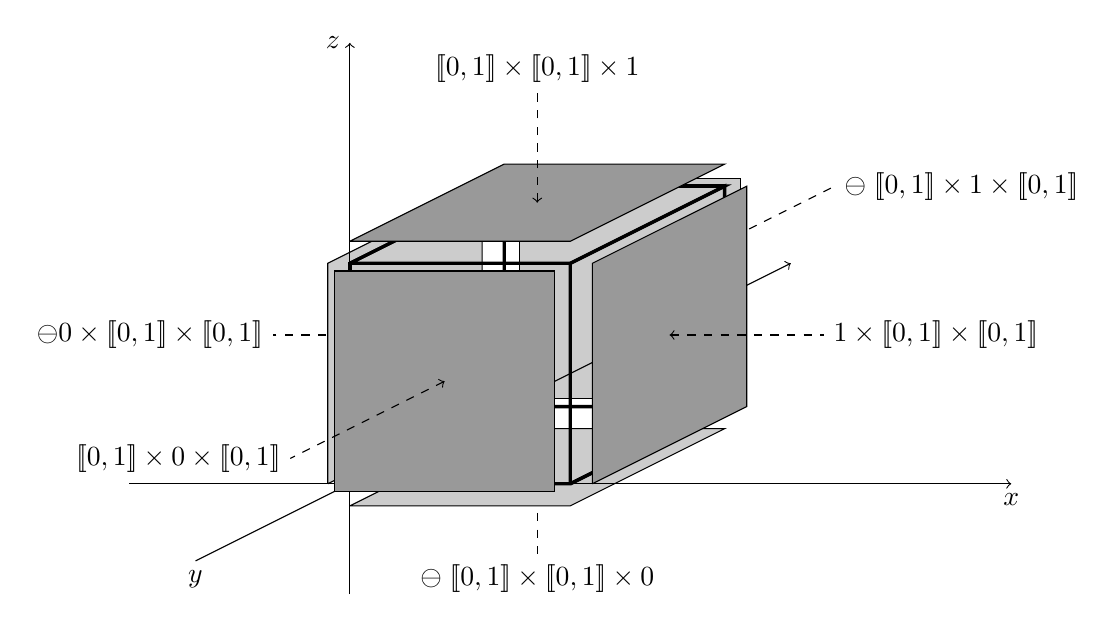
\begin{tikzpicture}[y=1.4cm, x=2.8cm]	
 	%axis
 	
 	%left
	\draw[color=black, dashed, <-] (0.35, 1.35) --++ (-0.7, 0) node[anchor=east, black] {$\ominus \hset{0} \times [\![0,1]\!] \times [\![0,1]\!]$};
	%back
	\draw[color=black, dashed, <-] (1.2,1.7) --++ (1,1) node[anchor=west, black] {$\ominus \; [\![0,1]\!] \times \hset{1} \times [\![0,1]\!]$};
	%bottom
	\draw[color=black, dashed, <-] (0.85,0.35) --++ (0,-1) node[anchor=north, black] {$\ominus \; [\![0,1]\!] \times [\![0,1]\!] \times \hset{0}$};
 	
 	\filldraw[fill=black!20] (0,-0.2) --++ (1,0) --++ (0.7,0.7) --++ (-1,0) --++ (-0.7,-0.7);
	\filldraw[fill=black!20] (0.77,0.77) --++ (1,0) --++ (0,2) --++ (-1,0) --++ (0, -2);
	\filldraw[fill=black!20] (-0.1,0) --++ (0,2) --++ (0.7,0.7) --++ (0,-2) --++ (-0.7,-0.7);
 	
	\draw[->] (-1,0) -- coordinate (x axis mid) (3,0) node[anchor=north] {$x$};
    	\draw[->] (0,-1) -- coordinate (y axis mid) (0,4) node[anchor=east] {$z$};
	\draw[->] (-0.7,-0.7) node[anchor=north] {$y$} --++ (2.7,2.7) ;
	
	\draw[very thick] (0,0) --++ (1,0) --++ (0.7,0.7) --++ (-1,0) --++ (-0.7,-0.7);
	\draw[very thick] (0.7,0.7) --++ (1,0) --++ (0,2) --++ (-1,0) --++ (0, -2);
	\draw[very thick] (0,0) --++ (0,2) --++ (0.7,0.7) --++ (0,-2) --++ (-0.7,-0.7);
	\draw[very thick] (0,2) --++ (1,0) --++ (0.7,0.7) --++ (-1,0) --++ (-0.7,-0.7);
	\draw[very thick] (0,0) --++ (1,0) --++ (0,2) --++ (-1,0) --++ (0, -2);
	\draw[very thick] (1,0) --++ (0,2) --++ (0.7,0.7) --++ (0,-2) --++ (-0.7,-0.7);
	
	\filldraw[fill=black!40] (0,2.2) --++ (1,0) --++ (0.7,0.7) --++ (-1,0) --++ (-0.7,-0.7);
	\filldraw[fill=black!40] (-0.07,-0.07) --++ (1,0) --++ (0,2) --++ (-1,0) --++ (0, -2);
	\filldraw[fill=black!40] (1.1,0) --++ (0,2) --++ (0.7,0.7) --++ (0,-2) --++ (-0.7,-0.7);

	%right
	\draw[color=black, dashed, <-] (1.35+0.1, 1.35) --++ (0.7, 0) node[anchor=west, black] {$\hset{1} \times [\![0,1]\!] \times [\![0,1]\!]$};
	%front
	\draw[color=black, dashed, <-] (0.5-0.07,1-0.07) --++ (-0.7,-0.7) node[anchor=east, black] {$[\![0,1]\!] \times \hset{0} \times [\![0,1]\!]$};
	%top
	\draw[color=black, dashed, <-] (0.85,2.35+0.2) --++ (0,1) node[anchor=south, black] {$[\![0,1]\!] \times [\![0,1]\!] \times \hset{1}$};
\end{tikzpicture}
\end{figure}

There are several ways to interpret and visualize the $\oplus$ and $\ominus$ sign associated with each face.
Most naturally in $\mathbb{R}^3$ for 2-rectangles is to give each a front and back side with the sign determining which to use.
Alternatively, a 2-rectangle has a boundary formed by 1-rectangles which when drawn as arrows, will all meet head-to-tail.
This induces a clockwise or counter-clockwise cycle around the edge of the rectangle and so $\circlearrowright$ and $\circlearrowleft$ are also commonly used.
This can be seen in Figure 4.4.
One may even notice that the normals produced by both are the same and choose to use that.
These are all conceptual tools, which are convenient to use particularly in $\mathbb{R}^2$ and $\mathbb{R}^3$.
There may not be such a nice physical interpretation in other spaces.


\begin{figure}[ht]
\caption[Orientations of 2-rectangles]{One way of visualizing the orientation of 2-rectangles using clockwise and counter-clockwise cycles of arrows for 1-rectangles. 
The boundary of $[\![a,b]\!] \times [\![c,d]\!]$ becomes the cycle: 
$(a,c) \to (b,c) \to (b,d) \to (a,d) \to (a,c)$.
Showing the relationship between $[\![a,b]\!] \times [\![c,d]\!]$ and $[\![b,a]\!] \times [\![d,c]\!]$ }
\centering
\begin{tikzpicture}

	\def\rectCycle#1#2#3#4{
		\draw[thick, ->, color=black!80] (#1,#2) -- (#3,#2);
		\draw[thick, ->, color=black!60] (#3,#2) -- (#3,#4);
		\draw[thick, ->, color=black!40] (#3, #4) -- (#1,#4);
		\draw[thick, ->, color=black!20] (#1,#4) -- (#1,#2);
		\draw[thick, ->] (#1, 0) -- (#3, 0);
		%\draw[fill] (#1,#2) circle (1 pt);
	}

	
	\rectCycle {0+1}{1} {0+2}{2};
	\draw[<->] (0,3) -- (0,0) -- (3,0);
	\draw[very thick, ->] (0,1) -- (0,2);
	\draw (0,1.5) node[anchor=east] {$+$};
	\draw (1.5,0) node[anchor=north] {$+$};
	%\draw (1.5, 1.5) node {$+$};
	\draw(1.5,1.5) node {$\;\circlearrowleft^+$};
	
	  
	\rectCycle {4+2}{1} {4+1}{2};
	\draw[<->] (4+0,3) -- (4+0,0) -- (4+3,0);
	\draw[very thick, ->] (4+0,1) -- (4+0,2);
	\draw (4+0,1.5) node[anchor=east] {$+$};
	\draw (4+1.5,0) node[anchor=north] {$-$};
	%\draw (4+1.5, 1.5) node {$-$};
	\draw(4+1.5,1.5) node {$\;\circlearrowright^-$};
	
	
	\rectCycle {8+2}{2} {8+1}{1};
	\draw[<->] (8+0,3) -- (8+0,0) -- (8+3,0);
	\draw[very thick, ->] (8+0,2) -- (8+0,1);
	\draw (8+0,1.5) node[anchor=east] {$-$};
	\draw (8+1.5,0) node[anchor=north] {$-$};
	%\draw (8+1.5, 1.5) node {$+$};
	\draw(8+1.5,1.5) node {$\;\circlearrowleft^+$};
	
	
	\rectCycle {12+1}{2} {12+2}{1};
	\draw[<->] (12+0,3) -- (12+0,0) -- (12+3,0);
	\draw[very thick, ->] (12+0,2) -- (12+0,1);
	\draw (12+0,1.5) node[anchor=east] {$-$};
	\draw (12+1.5,0) node[anchor=north] {$+$};
	%\draw (12+1.5, 1.5) node {$-$};
	\draw(12+1.5,1.5) node {$\;\circlearrowright^-$};
\end{tikzpicture}
\end{figure}


%%%%%%%%%%%%%%%%%%%%%%%%%%%%%%%%%%%%%%%%%
%
% CHAINS
%
%%%%%%%%%%%%%%%%%%%%%%%%%%%%%%%%%%%%%%%%%
\section{Chains}

In fact, we have already seen $k$-chains without mentioning them explicitly.
The boundary of a $k$-cube was the sum $\oplus$, of $2k$ $(k-1)$ cubes.
Chains do not have to be boundaries however, any linear combination of $k$-cubes will do.


\begin{definition}
We denote the Abelian group of of all $k$-cubes in $X$ as $C_k(X)$ (omitting $X$ when obvious by context).
An element $c \in C_k$(X) is called a \textbf{$\boldsymbol{k}$-chain on $X$} and is of the form:
\begin{equation}
	c = \bigoplus_{c_i \in X} \lambda_i c_i
\end{equation}
with integer coefficients $\lambda_i$ and  $k$-cubes in $c_i$.
If coefficients $\lambda_i$ are $\pm 1$ and $c$ is \emph{locally finite} (i.e. each $c_i$ intersects with only finitely many $c_j$ that have non-zero coefficients) then we say that $c$ is a \textbf{domain of integration}.
\end{definition}


		
Since $k$-chains are just linear combinations of $k$-cubes, we naturally extend many of our definitions linearly as well.
The integral $\int_c f$ of a $k$-chain $c=\bigoplus_i \lambda_i c_i$ is defined as $\lambda_i \int_{c_i} f  + \lambda_2 \int_{c_2} f + \ldots$.
Doing the same for the boundary operator $\partial$ we have:
\begin{align*}
	&\partial_k: C_k \to C_{k-1} \\
	&\partial_k(c) = \bigoplus_{i=1}^k \lambda_i \partial_k(c_i)
\end{align*}
Elegantly, the boundary operator now maps $k$-chains to $(k-1)$-chains!
\begin{equation}
	\ldots \xleftarrow{\partial_{k-1}} C_{k-1} \xleftarrow{\partial_{k}} C_k \xleftarrow{\partial_{k+1}} C_{k+1} \xleftarrow{\partial_{k+2}} ...
\end{equation}
The most natural next question becomes \emph{``What does $\partial_{k-1}( \partial_k ( c ))$ look like?''}




%%%%%%%%%%%%%%%%%%%%%%%%%%%%%%%%%%%%%%%%%
% BOUNDARY OF A BOUNDARY
%%%%%%%%%%%%%%%%%%%%%%%%%%%%%%%%%%%%%%%%%
\subsection{Example: \emph{Boundary of a boundary (of a 2-cube)}}
Let $\boldsymbol{a} =(a_1,a_2)$ and $\boldsymbol{b}= (b_1,b_2)$.
We wish to compute $\partial_1 ( \partial_2 ( \; [\![\boldsymbol{a}, \boldsymbol{b} ]\!] \; ) )$
\begin{align}
	\partial_1 ( \partial_2 ( [\![ a_1 , b_1 ]\!] \times [\![a_2, b_2 ]\!] ) )
	=	& 	\; \ominus 	\partial_1( \hset{0} \times [\![0,1]\!]) 
			\; \oplus \; 	\partial_1(\hset{1} \times [\![0,1]\!]) \notag \\
		& 	\; \oplus 	\partial_1( [\![0,1]\!] \times \hset{0}) 
			\; \ominus \; \partial_1([\![0,1]\!] \times \hset{1}) \\
	=	& 	\ominus	( 	\ominus \hset{(0,0)} \oplus \hset{(0,1)} ) 
			\;\oplus\;(	\ominus \hset{(1,0)} \oplus \hset{(1,1)}) \notag \\
		& 	\oplus ( 		\ominus \hset{(0,0)} \oplus \hset{(1,0)} ) 
			\;\ominus\;(	\ominus \hset{(0,1)} \oplus \hset{(1,1)}) \\
	=	& \;\emptyset	
\end{align}


When moving from (4.21) to (4.22), in addition to applying $\partial_1$ we also simplify, $\hset{x} \times \hset{y} = \hset{ (x,y) }$.
The identity ``$\partial \partial = 0$'' is not unique to $2$-cubes but holds for higher dimensions as well.


\begin{figure}[ht]
\caption[Boundary of a boundary (of a 2-cube)]{The boundary of 2-cube gives a cycle of oriented edges. Taking the boundary of again, at each corner, the negative boundary of one edge will be canceled by the positive boundary of the preceding edge.}
\centering
	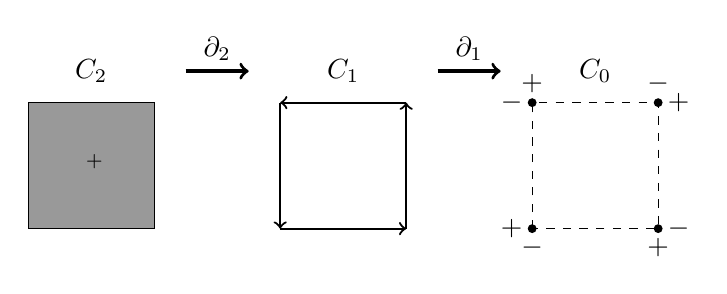
\begin{tikzpicture}[scale=0.8]
	
		\draw (1,2.5) node {$C_2$};
		\filldraw[fill=black!40] (0,0) rectangle (2,2);
		\draw (1,1) node {$\;\circlearrowleft^+$};
		
		\draw[very thick, ->] (2.5,2.5) --++ (0.5,0) node[anchor=south] {$\partial_2$} --++ (0.5,0);
		
		\draw (4+1,2.5) node {$C_1$};
		\draw[thick, ->] (4+0,0) --++ (2,0);
		\draw[thick, ->] (4+2,0) --++ (0,2);
		\draw[thick, ->] (4+2,2) --++ (-2,0);
		\draw[thick, ->] (4+0,2) --++ (0,-2);
		
		\draw[very thick, ->] (6.5,2.5) --++ (0.5,0) node[anchor=south] {$\partial_1$} --++ (0.5,0);
		
		\draw (8+1,2.5) node {$C_0$};
		\draw[dashed] (8+0,0) --++ (0,2) --++ (2,0) --++ (0,-2) --++ (-2,0);
		\fill (8,0) node[anchor=north] {$-$} node[anchor=east] {$+$} circle (2pt);
		\fill (8+2,0) node[anchor=west] {$-$} node[anchor=north] {$+$}  circle (2pt);
		\fill (8+2,2) node[anchor=south] {$-$} node[anchor=west] {$+$} circle (2pt);
		\fill (8,2) node[anchor=east] {$-$} node[anchor=south] {$+$} circle (2pt);
		
	\end{tikzpicture}
\end{figure}


Let $[\![\boldsymbol{a}, \boldsymbol{b}]\!]$ be a $k$-rectangle in $\mathbb{R}^n$.
Then we have:
\begin{align}
	\partial_k \partial_{k-1} \left( [\![ \boldsymbol{a}, \boldsymbol{b} ]\!] \right) 
	= \bigoplus_{j=1}^k (-1)^j 
		& \;  \left( \; \partial_{n-1} \left(	
			[\![ 	\boldsymbol{a}^{[\![1,n]\!]}, \;\;
				\boldsymbol{b}^{[\![1,i_j)\!)}
					\oplus \boldsymbol{a}^{[\![i_j]\!]}
					\oplus \boldsymbol{b}^{(\!(i_j,n]\!]} 
			]\!] 
		\right) \right. \notag\\[-1em]
		& \ominus \; \left. \! \partial_{n-1} \left(
			[\![ 	\boldsymbol{a}^{[\![1,i_j)\!)}
					\oplus \boldsymbol{b}^{[\![i_j]\!]}
					\oplus \boldsymbol{a}^{(\!(i_j,n]\!]} , \;\;
				\boldsymbol{b}^{[\![1,n]\!]}
			]\!] 
		\right)\right) \\[1em]
	= \bigoplus_{j=1}^k \bigoplus_{\ell=1}^{k-1} (-1)^{j+\ell}
		\;&
			[\![ 	(\boldsymbol{a}^{[\![1,n]\!]}), \;\;
				(\boldsymbol{b}^{[\![1,i_j)\!) \;\oplus\; (\!(i_j,i_{j,\ell})\!) \;\oplus\; (\!(i_{j,\ell},n]\!]}
					\oplus \boldsymbol{a}^{[\![i_j]\!] \;\oplus\; [\![i_{j,\ell}]\!]})
			]\!] \notag\\[-1em]
		\ominus \;&
			[\![ 	(\boldsymbol{a}^{[\![1,i_{j,\ell})\!) \;\oplus\; (\!(i_{j,\ell},n]\!]}
					\oplus \boldsymbol{b}^{[\![i_{j,\ell}]\!]}), \;\;
				(\boldsymbol{b}^{[\![1,i_j)\!) \;\oplus\; (\!(i_j,n]\!]}
					\oplus \boldsymbol{a}^{[\![i_j]\!]})
			]\!] \notag\\
		\ominus \; &
			[\![ 	(\boldsymbol{a}^{[\![1,i_j)\!) \;\oplus\; (\!(i_j,n]\!]}
					\oplus \boldsymbol{b}^{[\![i_j]\!]}), \;\;
				(\boldsymbol{b}^{[\![1,i_{j,\ell})\!) \;\oplus\; (\!(i_{j,\ell},n]\!]}
					\oplus \boldsymbol{a}^{[\![i_{j,\ell}]\!]})
			]\!] \notag\\
		\oplus \;&
			[\![ 	(\boldsymbol{a}^{[\![1,i_j)\!) \;\oplus\; (\!(i_j,i_{j,\ell})\!) \;\oplus\; (\!(i_{j,\ell},n]\!]}
					\oplus \boldsymbol{b}^{[\![i_j]\!] \;\oplus\; [\![i_{j,\ell}]\!]}), \;\;
				(\boldsymbol{b}^{[\![1,n]\!]})
			]\!] 
\end{align}
Note that we have $i_j$ and $i'_\ell$; after applying the first boundary operator, one dimension of the $k$-cube is degenerate.
Hence for each sequence: $\{i_j\}_{j=1}^k$ we construct $\{i_{j,\ell}\}_{\ell=1}^{k-1}$ given by:
\begin{equation}
	i_{j,1} , \ldots, i_{j,k-1} = i_1, \ldots, \widehat{i_j}, \ldots, i_k
\end{equation}
The double sum iterates over all pairs but $\oplus$ commutes so the $(k-2)$-cube with degenerate dimensions $[\![i_j]\!] \oplus [\![i_{j,\ell}]\!]$ will be iterated over twice. 
The sequences depend on one another so it is not as simple as simply swapping $\ell$ and $j$:
\begin{equation}
   [\![i_j]\!] \oplus [\![i_{j,\ell}]\!] =
     \begin{cases}
       [\![i_\ell]\!] \oplus [\![i_{\ell,j-1}]\!] & j > \ell \\
       [\![i_{\ell+1}]\!] \oplus [\![i_{\ell+1,j}]\!] & j \leq \ell
     \end{cases}
\end{equation}


So each term representing a $(k-2)$-cube will occur twice in the sum.
Once with the iteration $(j,\ell)$ and once with $(\ell, j-1)$ or $(\ell+1, j)$.
In either case, $(-1)^{j+\ell}$ is inverted meaning the two cubes will cancel.
Leaving us with the boundary of a boundary being empty.
By linearity this extends to all chains as well as the sum of empty sets is of course still empty.





%%%%%%%%%%%%%%%%%%%%%%%%%%%%%%%%%%%%%%%%%
%
% STOKE'S THEOREM
%
%%%%%%%%%%%%%%%%%%%%%%%%%%%%%%%%%%%%%%%%%
\section{Stokes' Theorem}


This result mirrors the earlier $\diff \diff = 0$ and this duality goes deeper.
The boundary $\partial$ maps a $k+1$-chain to a $k$-chain while 
the exterior derivative $\diff$ mapped a $k$-form to a $k+1$-form.
Sometimes this is written out as:
\begin{equation*}
	\ldots 	\xleftarrow{\partial} C_{k-1} 
			\xleftarrow{\partial} C_k 
			\xleftarrow{\partial} C_{k+1} 
			\xleftarrow{\partial} \ldots
\end{equation*}
\begin{equation*}
	\ldots 	\xrightarrow{\diff} \Lambda^{k-1} 
			\xrightarrow{\diff} \Lambda^k 
			\xrightarrow{\diff} \Lambda^{k+1} 
			\xrightarrow{\diff} \ldots
\end{equation*}
Stokes' Theorem is an important result which links the two even closer and generalizes many classical theorems including
the fundamental theorem of calculus, Green's theorem and the divergence theorem.


Given a $k-1$-form $\omega$ and $k$ chain $M$:
\begin{equation}
	\tag{Stokes' Theorem}
	\int_{\partial M} \omega = \int_M d\omega
\end{equation}


\begin{proof}

First we will consider Stokes theorem for the standard cube $I^k = [0,1]^k \subset \mathbb{R}^k$.
In the previous section we saw how cumbersome representing the faces in $\partial I^k$, could be.
We will denote the faces of $I^k$ by $I^k_{i=0}$ and $I^k_{i=1}$ for the $i$-th faces of $I^k$.
This allows us to rewrite the boundary more succinctly as:


\begin{equation}
	\partial (I^k) = \bigoplus_{i=1}^k (-1)^i \left( I^k_{i=0} \ominus I^k_{i=1} \right) 
\end{equation}



A $k-1$-form $\omega$ can be written as the sum
\begin{equation}
	\omega 
		= \sum_{i=1}^k \omega_i 
		= \sum_{i=1}^k f_i \; dx_1 \wedge \ldots \wedge \widehat{dx_i} \wedge  \ldots \wedge dx_k
\end{equation}
but since everything: the integrals, $d$ and $\partial$ are all linear, we can work using just one of these terms.
Assuming Stokes' theorem holds for $\omega_i$ then we immediately have it for $\omega$ as well:
\begin{align*}
	\int_{\partial\Omega} \omega 
	&= \int_{\partial \Omega} (\omega_1 + \ldots + \omega_k) \\
	&= \int_{\partial\Omega} \omega_1 + \ldots + \int_{\partial\Omega} \omega_k  \\
	&= \int_{\Omega} d\omega_1 + \ldots + \int_\Omega d\omega_k \\
	&= \int_\Omega (d\omega_1 + \ldots + d\omega_k)\\
	&= \int_\Omega d(\omega_1 + \ldots + \omega_k) = \int_\Omega d\omega
\end{align*}



To compute $d\omega$, we have for each term in the sum:
\begin{align*}
	d \left( f_i dx_1 \wedge \ldots \wedge \widehat{dx_i} \wedge  \ldots \wedge dx_k \right) 
 		&= df_i \wedge dx_1 \wedge \ldots \wedge \widehat{dx_i} \wedge  \ldots \wedge dx_k \\ 
 		&= \left( \sum_{j=1}^k \frac{\partial f_i}{\partial x_j} dx_j \right)
 			\wedge dx_1 \wedge \ldots \wedge \widehat{dx_i} \wedge  \ldots \wedge dx_k
\end{align*}
But for $j \neq i$, there will be a duplicate $dx_j$ term and this collision will cause the term to go to zero.
Hence only one term in the sum, $i=j$ will actually result in a non-zero term:
\begin{align*}
	d \left( f_i dx_1 \wedge \ldots \wedge \widehat{dx_i} \wedge  \ldots \wedge dx_k \right) 
 		&= \left(\frac{\partial f_i}{\partial x_i} dx_i \right)
 			\wedge dx_1 \wedge \ldots \wedge \hat{dx_i} \wedge  \ldots \wedge dx_k \\ 
		&= (-1)^{i-1} \frac{\partial f_i}{\partial x_i}
 			 dx_1 \wedge \ldots \wedge dx_k
\end{align*}



Since this is an integral over the canonical basis $\text{x} = (x_1, \ldots, x_k)$ we can remove the wedge products and
integrate as normal.
\begin{align*}
	\int_{[0,1]^k} d\omega_i
		=&\; (-1)^{i-1} \int_{[0,1]^k} \frac{\partial f_i}{\partial x_i}\; d(x_1, \ldots, x_k) \\
		=&\; (-1)^{i-1} \int_{[0,1]^{k-1}} \left( \int_0^1 \frac{\partial f_i}{\partial x_i} dx_i \right) 
			\;d(x_1, \ldots, \widehat{x_i}, \ldots, x_k)\\
		=&\; (-1)^{i-1}\left( \int_{[0,1]^{k-1}} f_i(x_1, \ldots, x_{i-1}, 1, x_{i+1}, \ldots, x_k)
			\;d(x_1, \ldots, \widehat{x_i}, \ldots, x_k) \right.\\
		&\;	- \left. \int_{[0,1]^{k-1}} f_i(x_1, \ldots, x_{i-1}, 0, x_{i+1}, \ldots, x_k)
			\;d(x_1, \ldots, \widehat{x_i}, \ldots, x_k) \right)
\end{align*}
The trick here being Fubini's Theorem allowing us to evaluate the iterated integral in whichever order we choose.
On the other side of the equality we have:
\begin{align*}
	\int_{\partial I^k} \omega_i
		&= \sum_{j=1}^k (-1)^j \int_{I^k_{j=0}} \omega_i - \int_{I^k_{j=1}} \omega_i
\end{align*}
but $I^k_{j=0}$ is just a $k-1$-rectangle embedded in $\mathbb{R}^k$ by the map:
\begin{equation*}
	(x_1, \ldots x_{k-1}) \mapsto (x_1, \ldots, x_{j-1}, 0, x_{j}, \ldots x_{k-1})
\end{equation*}
So we could alternatively think of $I^k_{j=0}: I^{k-1} \to I^k$ as just a change in coordinates:
\begin{align*}
	\int_{\partial I^k} \omega_i 
		=&\; \sum_{j=1}^k (-1)^j 
			\left(\int_{I^{k-1}} (I^k_{j=0})^*\omega_i - \int_{I^{k-1}} (I^k_{j=1})^* \omega_i \right) \\
		=&\; \sum_{j=1}^k (-1)^j 
			\left(\int_{I^{k-1}} f_i (x_1, \ldots, x_{i-1}, 0, x_{i+1}, \ldots, x_k)
				\;dx_1 \wedge \ldots \wedge \widehat{dx_i} \wedge  \ldots \wedge dx_k \right. \\
		&	\left. - \int_{I^{k-1}} f_i (x_1, \ldots, x_{i-1}, 1, x_{i+1}, \ldots, x_k)
				\;dx_1 \wedge \ldots \wedge \widehat{dx_i} \wedge  \ldots \wedge dx_k \right)\\
		=&\; (-1)^i \left(\int_{I^{k-1}} f_i (x_1, \ldots, x_{i-1}, 0, x_{i+1}, \ldots, x_k)
				\;d(x_1, \ldots,\widehat{x_i},  \ldots, x_k) \right. \\
		&	\left. - \int_{I^{k-1}} f_i (x_1, \ldots, x_{i-1}, 1, x_{i+1}, \ldots, x_k)
				\;d(x_1, \ldots,\widehat{x_i},  \ldots, x_k) \right)
\end{align*}



In the final step we observe that all terms in the sum for $i \neq j$ end up disappearing leaving us with just the term for
$i=j$.
Clearly, both sides of the equation are the same and so Stokes' theorem holds for the standard cube.
From here, the remaining cases build on one another are quite straight-forward.
For a singular cube $c$, we have:
\begin{align*}
	\int_{\partial c} \omega
		&= \int_{c (\partial ([0,1]^k))} \omega \\
		&= \int_{\partial( [0,1]^k)} c^* \omega \\
		&= \int_{[0,1]^k} dc^* \omega \\
		&= \int_{[0,1]^k} c^* d \omega \\
		&= \int_c d\omega
\end{align*}
And for a chain $C=a_1 c_1 + \ldots + a_n c_n$ made up of singular cubes:
\begin{align*}
	\int_C d\omega 
		&= \int_{a_1c_1 + \ldots + a_nc_n	} d\omega \\
		&= a_1 \int_{c_1} d\omega + \ldots + a_n \int_{c_n} d\omega \\
		&= a_1 \int_{\partial c_1} \omega + \ldots + a_n \int_{\partial c_n} \omega \\
		&= \int_{a_1 \partial c_1 + \ldots a_n \partial c_n} \omega \\
		&= \int{\partial ( a_1c_1 + \ldots + a_n c_n)} \omega \\
		&= \int_{\partial C} \omega
\end{align*}

And so we have Stokes' theorem on general chains.
\end{proof}


%%%%%%%%%%%%%%%%%%%%%%%%%%%%%%%%%%%%%%%%%
% CONTOUR EXAMPLE
%%%%%%%%%%%%%%%%%%%%%%%%%%%%%%%%%%%%%%%%%
\subsection{Example: \emph{Contour Integral}}


Generalized partitions can extend past the original domain but so far this has been done through relatively
obvious extensions.
Sometimes the additional regions that are added and negated can be quite unexpected.
\emph{Contour integration} is a method for solving integrals that can involve the usage of curious looking regions to solve.
Consider the following function defined on the real numbers:
\begin{equation}
	f(x) = \frac{1}{x^4 + 1}
\end{equation}
and suppose we wish to compute the integral over the entire real line:
\begin{equation}
	 \int_{-\infty}^\infty f(x) \diff x
\end{equation}
This is a difficult integral to evaluate directly so instead of treating $f$ as a real function, $f:\mathbb{R} \to \mathbb{R}$, 
we instead consider it as a complex function: $f:\mathbb{C} \to \mathbb{C}$.


Let $C_1$ be the straight line curve from $-r$ to $r$: $C_1(t) =rt-(1-t)r$ and
$C_2$ the circular arc with radius $r$ from $r$  to $-r$: $C_2(t) = re^{it}$.
Finally let $C$ the combined curve: $C= C_1 \oplus C_2$
Then our desired value is the integral over $C_1$ as $r$ goes to infinity:
\begin{equation}
	\int_{C_1} f(x) \diff x = \oint_{C} f(z) \diff z - \int_{C_2} f(z) \diff z
\end{equation}


\begin{figure}[ht]
	\caption[Contour Integral]{The contours $C_1$ and $C_2$ and with the four singularities of $f$ marked.}
	\label{fig:contourintegration}
	\centering
	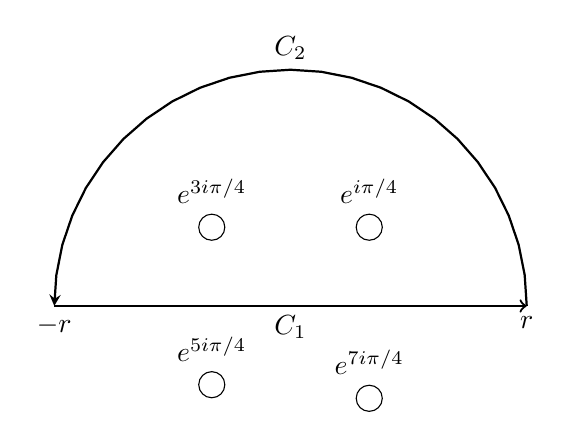
\begin{tikzpicture}
		\draw[>=stealth, thick, ->, domain=0:180] plot ({3*cos(\x)}, {3*sin(\x)});
		\draw[thick, <-] (3,0) node[below] {$r$} -- (-3,0) node[below] {$-r$};
		\node[draw,circle,label=$e^{i \pi/4}$] at (1,1) {};
		\node[draw,circle,label=$e^{3 i \pi/4}$] at (-1,1) {};
		\node[draw,circle,label=$e^{5 i \pi/4}$] at (-1,-1) {};
		\node[draw,circle,below,label=$e^{7 i \pi/4}$] at (1,-1) {};
		\draw (0,3) node[above] {$C_2$};
		\draw (0,0) node[below] {$C_1$};
	\end{tikzpicture}
\end{figure}

To solve the integral on $C$ we can use the Cauchy residue theorem: a special case of the generalized Stokes' theorem.
$C$ is a closed simple path and $f$ is holomorphic everywhere except for a finite set of points $\{a_k\}_{i=1}^n$
and so we have:
\begin{equation}
	\oint_C f(z) \diff z = 2 \pi i \sum_{k=1}^n \Res(f, a_k)
\end{equation}
And so we must compute the residues of the two singularities above the real line: 
$W_8^1 = e^{i\pi/4}$ and $W_8^3 = e^{3i\pi/4}$.
These are both simple poles and can be computed as follows:
\begin{equation*}
	\Res(f, W_8^1) =\lim_{z \to W_8^1} \frac{z - W_8^1}{z^4 +1} 
		= \lim_{z \to W_8^1} \frac{1}{4z^3}
		= (1/4) W_8^{-3} = (1/4) W_8^5
\end{equation*}
\begin{equation*}
	\Res(f, W_8^3) =\lim_{z \to W_8^3} \frac{z - W_8^3}{z^4 +1} 
		= \lim_{z \to W_8^3} \frac{1}{4z^3}
		= (1/4) W_8^{-9} = (1/4) W_8^7
\end{equation*}
Converting these out of polar coordinates, we have 
	$W_8^7 = \left( \frac{\sqrt{2}}{2}-\frac{\sqrt{2}}{2}i \right)$ 
	and $W_8^5 =\left( -\frac{\sqrt{2}}{2}-\frac{\sqrt{2}}{2}i \right)$:
\begin{equation*}
	\oint_C f(z) \diff z 
	= 2 \pi i \left( 	\frac{1}{4} \left( \frac{\sqrt{2}}{2}-\frac{\sqrt{2}}{2}i \right) 
				+	\frac{1}{4} \left( -\frac{\sqrt{2}}{2}-\frac{\sqrt{2}}{2}i \right)\right)
	= \frac{\pi}{\sqrt{2}}
\end{equation*}
To compute the integral over $C_2$, we make the substitutions, $z = re^{i \theta}$ and $dz=ire^{i\theta} d\theta$:
\begin{equation*}
	\int_{C_2} f(z) \diff z = \int_0^\pi \frac{ire^{i\theta}}{r^4 e^{4i\theta} +1} \diff\theta
\end{equation*}
And then simply observe that as $r$ goes to infinity, this integral goes to zero and the term for $C_2$ drops off.
Leaving us with just:
\begin{equation*}
	\int_{-\infty}^\infty f(x) \diff x = \frac{\pi }{\sqrt{2}}
\end{equation*}

